\documentclass[12pt,letterpaper]{ntdhw}

\usepackage{framed}

\usepackage{ntdmath}

\usetikzlibrary{patterns}
\usetikzlibrary{decorations.pathreplacing}
\usetikzlibrary{decorations.pathmorphing}

\title{Project 2: SATPlan and the Tower of Hanoi}
\author{CSCI 561}


\rhead{Names: Luke Beukelman, Ben Breisch, Luc Lafave, Adam Thistlewood}

%\keytrue
\tikzset{
  hdisk/.style={
    rectangle,
    draw=black,
    minimum height=1em,
    minimum width=1.5em,
    inner sep=0,
    node distance=1em,
  },
  db/.style={
    node distance=.5em,
  },
  peg/.style={
    minimum width=.5em,
    minimum height=5em,
    node distance=2.5em,
    inner sep=0,
    rectangle,fill=black,
  },
  hd0/.style={
    hdisk,
    fill=red!10!white,
    minimum width=2em
  },
  hd1/.style={
    hdisk,
    fill=green!10!white,
    minimum width=3em
  },
  hd2/.style={
    hdisk,
    fill=blue!10!white,
    minimum width=4em
  },
  hd3/.style={
    hdisk,
    fill=purple!30!white,
    minimum width=5em
  },
  rewrite/.style = {%
    ->,very thick,decorate,%
    decoration={snake,
      post=lineto,post length=.5em,
      pre=lineto,pre length=.5em
    }
  }
}

% \tikzstyle{A} = [fill=red!10!white]
% \tikzstyle{B} = [fill=green!10!white]
% \tikzstyle{C} = [fill=blue!10!white]

\newcommand{\fbdground}[2] {%
  \draw (-#1/2,0)-- (#1/2,0); % line
  \fill[pattern=north east lines,name=ground] (-#1/2,0) rectangle (#1/2,-#2); % hashes
}

\begin{document}
\pagestyle{fancyplain}

\maketitle
\thispagestyle{fancyplain}
%\clearpage

\begin{leftbar}
  The \emph{Tower of Hanoi} is a classic puzzle consisting of round
  disks stacked on pegs.  One must move all disks to the final peg,
  subject to the following constraints:
  \begin{enumerate}
    \item Only one disk can be moved at a time.
    \item Each move consists of taking the upper disk from one of the
    stacks and placing it on top of another stack.
    \item No disk may be placed on top of a smaller disk.
  \end{enumerate}

 \noindent Answer the following questions:
\end{leftbar}

\begin{enumerate}
  \item  Create PDDL domains (operators and facts) for the following Tower of
  Hanoi instances (it is possible that the PDDL operators will be the
  same):
  \begin{enumerate}
    \item Two pegs and one disk. \\
    Operators (all same):
    \listpddl{hanoidomain.pddl}
    Facts:
    \listpddl{twopegsonedisk.pddl}
    \item Three pegs and two disks. \\
    Operators (all same):
    \listpddl{hanoidomain.pddl}
    Facts:
    \listpddl{threepegstwodisks.pddl}
    \item Three pegs and four disks. \\
    Operators (all same):
    \listpddl{hanoidomain.pddl}
    Facts:
    \listpddl{threepegsfourdisks.pddl}
  \end{enumerate}

  \item  Download one or more of the following planners and use them to
  produce plans for your PDDL domains:
  \begin{itemize}
    \item BlackBox:
    \url{https://gitlab.com/HenryKautz/BlackBox/}
    \item Madagascar:
    \url{http://research.ics.aalto.fi/software/sat/madagascar/}
    \item TMKit:
    \url{http://tmkit.dyalab.org/}
  \end{itemize}
  What plans are produced by each planner for each instance (one, two,
  four disks)?

    \begin{enumerate}
        \item Two Peg, One Disk \\
        \listpddl{onediskplan.pddl}
        \item Three Peg, Two Disk
        \listpddl{twodiskplan.pddl}
        \item Three Peg, Four Disk
        \listpddl{fourdiskplan.pddl}
    \end{enumerate}

    \item  Encode the three-peg, two-disk instance as a Boolean formula using the
    SATPlan method.  Please separately indicate the different parts of your
    encoding (start state, goal conditions, frame axioms, etc.).

  \item Find the satisfying assignments for the three-peg, two-disk
    Boolean formula using your DPLL implementation.
    \begin{enumerate}
    \item What is the satisfying assignment?
       \\Each needs to be true if not literal bound to false.
\\(NOOP\_SMALLER\_DISK1\_PEG3\mbox{-}1 
\\NOOP\_SMALLER\_DISK1\_PEG2\mbox{-}1 
\\NOOP\_SMALLER\_DISK2\_PEG3\mbox{-}2
\\NOOP\_SMALLER\_DISK2\_PEG2\mbox{-}1 
\\ON\_DISK1\_PEG2\mbox{-}1 
\\NOOP\_ON\_DISK1\_PEG2\mbox{-}2
\\(NOT ON\_DISK1\_PEG3\mbox{-}2) 
\\(NOT CLEAR\_PEG3\mbox{-}2) 
\\NOOP\_CLEAR\_DISK2\mbox{-}2
\\(NOT ON\_DISK1\_DISK2\mbox{-}1) 
\\(NOT ON\_DISK1\_DISK2\mbox{-}2) 
\\(NOT NOOP\_ON\_DISK1\_DISK2\mbox{-}1)
\\(NOT ON\_DISK2\_PEG1\mbox{-}2) 
\\(NOT CLEAR\_PEG2\mbox{-}1) 
\\(NOT ON\_DISK2\_PEG2\mbox{-}2)
\\(NOT NOOP\_CLEAR\_PEG2\mbox{-}1) 
\\(NOT NOOP\_CLEAR\_PEG3\mbox{-}2) 
\\NOOP\_ON\_DISK2\_PEG1\mbox{-}1
\\(NOT MOVEDISK\_DISK1\_PEG2\_PEG3\mbox{-}2) 
\\NOOP\_SMALLER\_DISK1\_DISK2\mbox{-}1
\\(NOT MOVEDISK\_DISK2\_PEG1\_PEG2\mbox{-}2) 
\\MOVEDISK\_DISK1\_DISK2\_PEG2\mbox{-}1
\\(NOT MOVEDISK\_DISK1\_PEG2\_DISK2\mbox{-}2) 
\\NOOP\_CLEAR\_DISK1\mbox{-}1
\\(NOT NOOP\_ON\_DISK2\_PEG1\mbox{-}2) 
\\NOOP\_SMALLER\_DISK2\_PEG3\mbox{-}1
\\(NOT MOVEDISK\_DISK1\_DISK2\_PEG3\mbox{-}2) 
\\CLEAR\_DISK2\mbox{-}1
\\(NOT MOVEDISK\_DISK1\_DISK2\_PEG2\mbox{-}2) 
\\SMALLER\_DISK2\_PEG3\mbox{-}1
\\(NOT NOOP\_ON\_DISK1\_DISK2\mbox{-}2) 
\\ON\_DISK2\_PEG1\mbox{-}1 
\\MOVEDISK\_DISK2\_PEG1\_PEG3\mbox{-}2
\\CLEAR\_DISK1\mbox{-}1
\\NOOP\_CLEAR\_DISK1\mbox{-}2 
\\SMALLER\_DISK1\_DISK2\mbox{-}1
\\NOOP\_SMALLER\_DISK1\_DISK2\mbox{-}2 
\\ON\_DISK2\_PEG3\mbox{-}2 
\\NOOP\_ON\_DISK2\_PEG3\mbox{-}3 
\\CLEAR\_DISK1\mbox{-}2
\\(NOT MOVEDISK\_DISK1\_PEG3\_DISK2\mbox{-}3)
\\SMALLER\_DISK1\_DISK2\mbox{-}2
\\(NOT MOVEDISK\_DISK2\_PEG1\_PEG3\mbox{-}3) 
\\ON\_DISK1\_PEG2\mbox{-}2 
\\(NOT NOOP\_ON\_DISK1\_DISK2\mbox{-}3)
\\CLEAR\_DISK2\mbox{-}2 
\\MOVEDISK\_DISK1\_PEG2\_DISK2\mbox{-}3 
\\(NOT MOVEDISK\_DISK1\_PEG3\_PEG2\mbox{-}2)
\\(NOT NOOP\_ON\_DISK1\_PEG3\mbox{-}2) 
\\(NOT MOVEDISK\_DISK1\_PEG3\_DISK2\mbox{-}2)
\\(NOT ON\_DISK1\_PEG3\mbox{-}1) 
\\(NOT MOVEDISK\_DISK1\_DISK2\_PEG3\mbox{-}1) 
\\NOOP\_CLEAR\_PEG3\mbox{-}1
\\CLEAR\_PEG3\mbox{-}1 
\\(NOT MOVEDISK\_DISK2\_PEG2\_PEG3\mbox{-}3) 
\\SMALLER\_DISK1\_PEG2\mbox{-}0
\\SMALLER\_DISK1\_PEG3\mbox{-}0 
\\SMALLER\_DISK1\_DISK2\mbox{-}0 
\\ON\_DISK1\_DISK2\mbox{-}0 
\\CLEAR\_DISK1\mbox{-}0
\\ON\_DISK2\_PEG1\mbox{-}0 
\\SMALLER\_DISK2\_PEG3\mbox{-}0
\\CLEAR\_PEG2\mbox{-}0 
\\SMALLER\_DISK2\_PEG2\mbox{-}0
\\ON\_DISK1\_DISK2\mbox{-}3 
\\CLEAR\_PEG3\mbox{-}0 
\\ON\_DISK2\_PEG3\mbox{-}3)
\item What is the corresponding plan?
  \\(NOOP\_SMALLER\_DISK1\_PEG3\mbox{-}1 
\\NOOP\_SMALLER\_DISK1\_PEG2\mbox{-}1 
\\NOOP\_SMALLER\_DISK2\_PEG3\mbox{-}2
\\NOOP\_SMALLER\_DISK2\_PEG2\mbox{-}1 
\\ON\_DISK1\_PEG2\mbox{-}1 
\\NOOP\_ON\_DISK1\_PEG2\mbox{-}2
\\NOOP\_CLEAR\_DISK2\mbox{-}2
\\NOOP\_ON\_DISK2\_PEG1\mbox{-}1
\\NOOP\_SMALLER\_DISK1\_DISK2\mbox{-}1
\\MOVEDISK\_DISK1\_DISK2\_PEG2\mbox{-}1
\\NOOP\_CLEAR\_DISK1\mbox{-}1
\\NOOP\_SMALLER\_DISK2\_PEG3\mbox{-}1
\\CLEAR\_DISK2\mbox{-}1
\\SMALLER\_DISK2\_PEG3\mbox{-}1
\\ON\_DISK2\_PEG1\mbox{-}1 
\\MOVEDISK\_DISK2\_PEG1\_PEG3\mbox{-}2
\\CLEAR\_DISK1\mbox{-}1
\\NOOP\_CLEAR\_DISK1\mbox{-}2 
\\SMALLER\_DISK1\_DISK2\mbox{-}1
\\NOOP\_SMALLER\_DISK1\_DISK2\mbox{-}2 
\\ON\_DISK2\_PEG3\mbox{-}2 
\\NOOP\_ON\_DISK2\_PEG3\mbox{-}3 
\\CLEAR\_DISK1\mbox{-}2
\\SMALLER\_DISK1\_DISK2\mbox{-}2
\\ON\_DISK1\_PEG2\mbox{-}2 
\\CLEAR\_DISK2\mbox{-}2 
\\MOVEDISK\_DISK1\_PEG2\_DISK2\mbox{-}3 
\\NOOP\_CLEAR\_PEG3\mbox{-}1
\\CLEAR\_PEG3\mbox{-}1 
\\SMALLER\_DISK1\_PEG2\mbox{-}0
\\SMALLER\_DISK1\_PEG3\mbox{-}0 
\\SMALLER\_DISK1\_DISK2\mbox{-}0 
\\ON\_DISK1\_DISK2\mbox{-}0 
\\CLEAR\_DISK1\mbox{-}0
\\ON\_DISK2\_PEG1\mbox{-}0 
\\SMALLER\_DISK2\_PEG3\mbox{-}0
\\CLEAR\_PEG2\mbox{-}0 
\\SMALLER\_DISK2\_PEG2\mbox{-}0
\\ON\_DISK1\_DISK2\mbox{-}3 
\\CLEAR\_PEG3\mbox{-}0 
\\ON\_DISK2\_PEG3\mbox{-}3)
    \end{enumerate}


\end{enumerate}

\begin{figure}
  \centering
  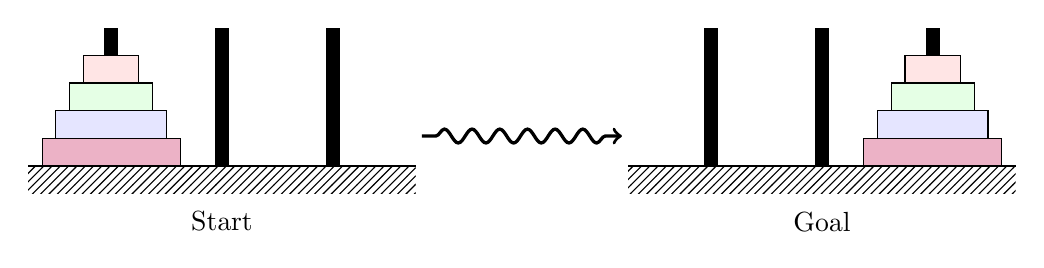
\begin{tikzpicture}
    \begin{scope}
      \fbdground{14em}{1em}

      \node[coordinate] at (-4em,0) (a0) {};
      \node[peg,above of=a0] {};

      \node[coordinate] at (0em,0) (b0) {};
      \node[peg,above of=b0] {};

      \node[coordinate] at (4em,0) (c0) {};
      \node[peg,above of=c0] {};

      \node[hd3,db,above of=a0] (3) {};
      \node[hd2,above of=3] (2) {};
      \node[hd1,above of=2] (1) {};
      \node[hd0,above of=1] (0) {};

      \node at (0,-2em) {Start};
    \end{scope}

    \draw (1in,.15in) edge[rewrite] (2in,.15in);

    \begin{scope}[xshift=3in]
      \fbdground{14em}{1em}

      \node[coordinate] at (-4em,0) (a0) {};
      \node[peg,above of=a0] {};

      \node[coordinate] at (0em,0) (b0) {};
      \node[peg,above of=b0] {};

      \node[coordinate] at (4em,0) (c0) {};
      \node[peg,above of=c0] {};

      \node[hd3,db,above of=c0] (3) {};
      \node[hd2,above of=3] (2) {};
      \node[hd1,above of=2] (1) {};
      \node[hd0,above of=1] (0) {};

      \node at (0,-2em) {Goal};
    \end{scope}
  \end{tikzpicture}

  \caption{Tower of Hanoi Puzzle with 3 pegs and 4 disks.}
\end{figure}

\end{document}


%%% Local Variables:
%%% mode: latex
%%% TeX-master: t
%%% End:
